\documentclass[a4paper,10pt]{jsarticle}
\usepackage{amsmath,amssymb}
\usepackage{bm}
\usepackage[dvipdfmx]{graphicx}
\usepackage[dvipdfmx]{color}

\title{Machine Learning Midterm Assignment}
\author{Keisuke Okumura, 18M31013}

\newcommand{\argmax}{\mathop{\rm argmax}\limits}
\newcommand{\argmin}{\mathop{\rm argmin}\limits}
\newcommand{\coloneq}{:=}

\begin{document}
\maketitle

\section*{Problem 1}
ロジスティック回帰では次の問題を解くことになる.
\[ \hat{\bm{w}} = \argmin_{\bm{w}}J(\bm{w}) \]
\[
 J(\bm{w}) \coloneq \sum_{i=1}^{n}(
 \ln{(1 + \exp{(-y_i\bm{w}^\mathrm{T}\bm{x}_i)}}))
 + \lambda \bm{w}^\mathrm{T}\bm{w}
\]

最急降下法(steepest gradient method)では, 以下の更新式に従って学習を行う. $\alpha$ は定数とする.
\[
\bm{w}^{(t+1)} = \bm{w}^{(t)} - \alpha\left.\frac{\partial J}{\partial \bm{w}}\right|_{\bm{w}=\bm{w}^{(t)}}
\]
\begin{align*}
\frac{\partial J(\bm{w})}{\partial \bm{w}}
 &= \frac{1}{n}\sum_{i=1}^{n}
 \frac{\exp(-y_i\bm{w}^\mathrm{T}\bm{x}_i)(-y_i\bm{x}_i)}
 {1 + \exp(-y_i\bm{w}^\mathrm{T}\bm{x}_i)}
 + 2\lambda\bm{w}\\
 &=\frac{1}{n}\sum_{i=1}^{n}
 \frac{-y_i\bm{x}_i}
 {1 + \exp(y_i\bm{w}^\mathrm{T}\bm{x}_i)}
 + 2\lambda\bm{w}\\
\end{align*}

また, ニュートン法(newton method)では以下の更新式に従って学習を行う. $\alpha$ は定数とする.
\[ \bm{w}^{(t+1)} = \bm{w}^{(t)} + \alpha\bm{d}^{(t)} \]
\[ \nabla^2J(\bm{w}^{(t)})\bm{d}^{(t)} = -\nabla J(\bm{w}^{(t)})
\Longleftrightarrow
\bm{d}^{(t)} = - (\nabla^2J(\bm{w}^{(t)}))^{-1} \nabla J(\bm{w}^{(t)})
\]

$\nabla^2J(\bm{w})$は次のように計算される.
\[
 \nabla^2J(\bm{w}) = \frac{1}{n}\sum_{i=1}^{n}
 \left(\frac{\exp(-y_i\bm{w}^\mathrm{T}\bm{x}_i)}
 {(1 + \exp(-y_i\bm{w}^\mathrm{T}\bm{x}_i))^2}\bm{x}_i\bm{x}_i^\mathrm{T}\right) + 2\lambda\bm{I}
\]

$100$個のデータからなるデータセットを Toy Dataset I\hspace{-1pt}I を参考に生成し,
最急降下法, 及びニュートン法を実行した結果を図.~\ref{img:log-result}に示す.
また, その時の学習の進行の様子を図.~\ref{img:log-loss}に示す.
パラメータ更新の繰り返し数は$50$回, $\alpha=0.1$, $\lambda=0.1$として学習を行った.

\begin{figure}[htbp]
 \begin{minipage}{0.5\hsize}
  \begin{center}
   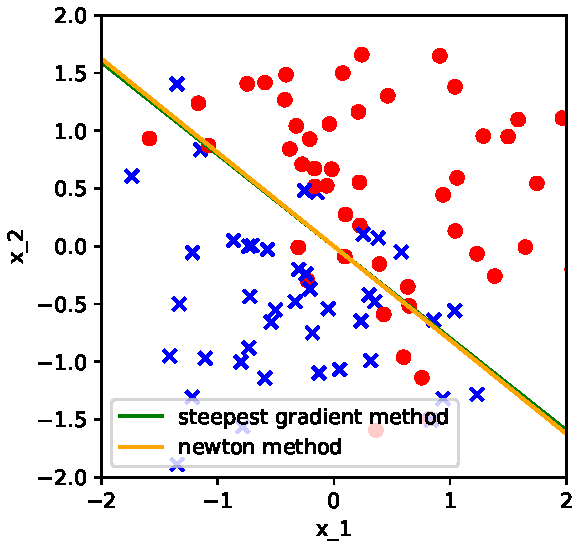
\includegraphics[width=7cm]{figs/p1_logistic-regression_result.pdf}
  \end{center}
  \caption{ロジスティック回帰の学習結果. $\bm{w}^\mathrm{T}\bm{x}=0$ を描画.}
  \label{img:log-result}
 \end{minipage}
 \begin{minipage}{0.5\hsize}
  \begin{center}
   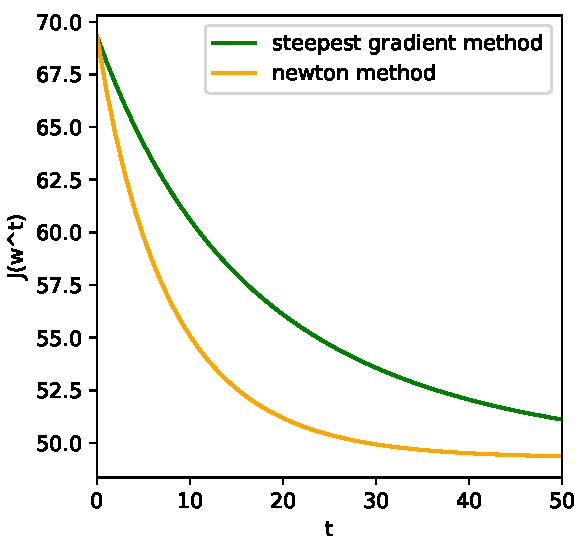
\includegraphics[width=7cm]{figs/p1_logistic-regression_loss.pdf}
  \end{center}
  \caption{損失関数の値の変化.}
  \label{img:log-loss}
 \end{minipage}
\end{figure}

\section*{Problem 2}
本問題では, \textit{lasso}を用いて次の問題を考える.
\[
 \hat{\bm{w}} = \argmin_{\bm{w}}((\bm{w}-\bm{\mu})^\mathrm{T}\bm{A}(\bm{w}-\bm{\mu})
 + \lambda||\bm{w}||_1)
\]
解を得るために, Proximal gradient methodを用いる.
$\psi = (\bm{w}-\bm{\mu})^\mathrm{T}\bm{A}(\bm{w}-\bm{\mu})$ とする.
更新式は次のようになる.
\begin{align*}
 w^{(t+1)}_i
 &= prox_{\eta_t\lambda||\cdot||_1}\left(\bm{w}^{(t)}
 - \eta_t\nabla\psi(\bm{w}^{(t-1)})\right)
\end{align*}
ここで, 学習率 $\eta_t=\gamma^{-1}$ とする.
$\gamma$ は $\psi$ のリプシッツ定数とし, $2\bm{A}$ の固有値の最大値をとることができる.
上式はL1ノルムの近接写像であるから, Soft Threshold関数を用いて, 次のように変換される.
\begin{align*}
 w^{(t+1)}_i
 = ST_{\frac{\lambda}{\gamma}}\left(w^{(t)}_i
 -\left\{\frac{1}{\gamma}\nabla\psi(\bm{w}^{(t)})\right\}_i\right),
 \,\,\,\,
 ST_q(\mu) = \begin{cases}
              \mu - q &(\mathit{if} \,\, \mu > q)\\
              0 &(\mathit{if} \,\, |\mu| \leq q)\\
              \mu + q &(\mathit{if} \,\, \mu < -q)\\
             \end{cases}
\end{align*}

$\psi$ を二次形式とみなし $\bm{A}$ を対称行列とすると, $\nabla \psi$ は次のようになる.
\[
 \nabla \psi = (\bm{A} + \bm{A}^\mathrm{T})(\bm{w} - \bm{\mu}) = 2\bm{A}(\bm{w} - \bm{\mu})
\]

以上より, 更新式は次式で表される.
\[
 w^{(t+1)}_i
 = ST_{\frac{\lambda}{\gamma}}\left(w^{(t)}_i
 -\left\{\frac{1}{\gamma}2\bm{A}(\bm{w}^{(t)} - \bm{\mu})\right\}_i\right)
\]

また, Accelerated proximal gradientを用いた場合, 更新式は次のように変化する.
\[
  \bm{w}^{(t+1)} = prox_{\eta_t\lambda||\cdot||_1}\left(
 \bm{v}^{(t)} - \eta_t\nabla\psi(\bm{v}^{(t)})\right)
\]
\[ \bm{v}^{(t)} = \bm{w}^{(t)} + q(t)(\bm{w}^{(t)} - \bm{w}^{(t-1)}) \]
$q(t)$はスカラー関数である. 今回は次式を用いる.
\[ q(t) = \frac{t-1}{t+2} \]

以上を踏まえて, 以下の条件で学習を行う.
\[
 \bm{A} = \left(\begin{array}{cc} 3 & 0.5 \\ 0.5 & 1 \end{array}\right), \,
 \bm{\mu} = \left(\begin{array}{c} 1 \\ 2 \end{array}\right)
\]

繰り返し数を$50$回, $\lambda$ を$2$, $4$, $6$と変えた時の学習の様子を図.~\ref{img:lasso-result}に示す.
さらに, 講義スライドを参照して $||\bm{w}^{(t)} - \hat{\bm{w}}||$ を計算し,
結果を図.~\ref{img:lasso-error}に示す.


\begin{figure}[htbp]
 \begin{minipage}{0.33\hsize}
  \begin{center}
   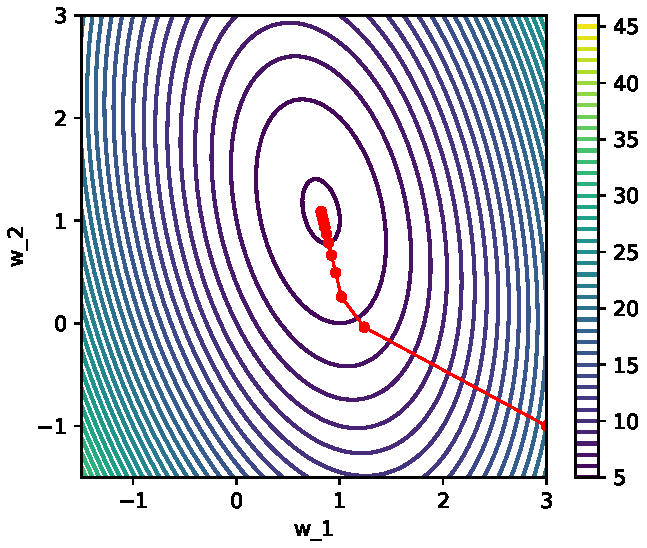
\includegraphics[width=5cm]{figs/p2_lasso_result_lambda-2.pdf}
  \end{center}
 \end{minipage}
 \begin{minipage}{0.33\hsize}
  \begin{center}
   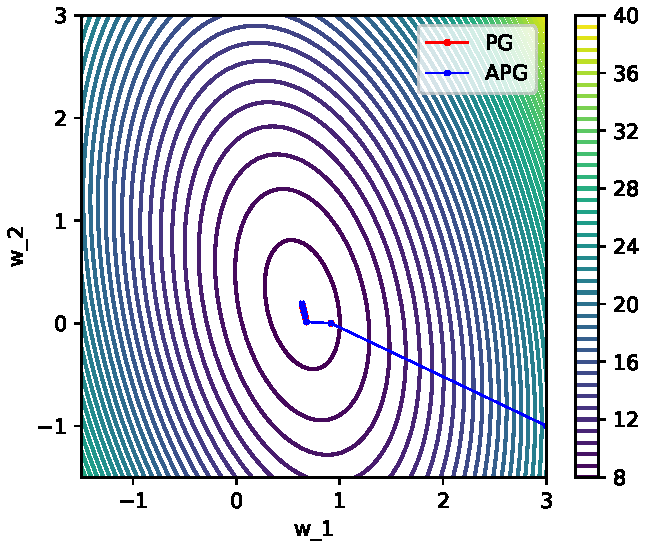
\includegraphics[width=5cm]{figs/p2_lasso_result_lambda-4.pdf}
  \end{center}
 \end{minipage}
 \begin{minipage}{0.33\hsize}
  \begin{center}
   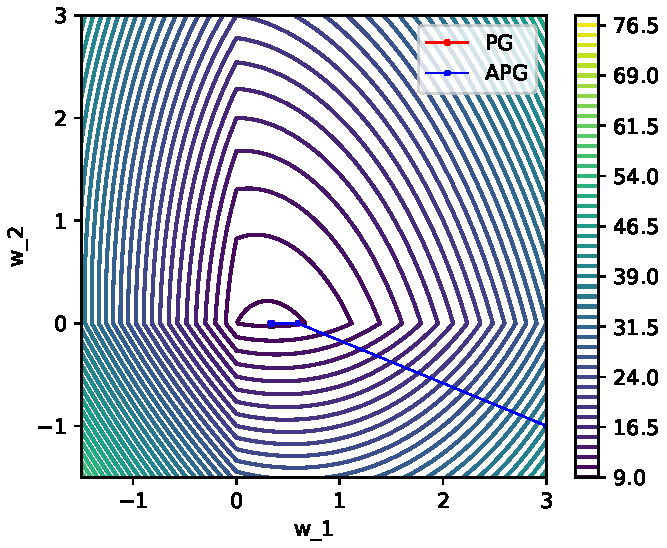
\includegraphics[width=5cm]{figs/p2_lasso_result_lambda-6.pdf}
  \end{center}
 \end{minipage}
 \caption{\textit{lasso}, Proximal gradientを用いて学習を行った様子. 
 左から $\lambda=2, 4, 6$となっている.}
 \label{img:lasso-result}
\end{figure}

\begin{figure}[htbp]
 \begin{center}
   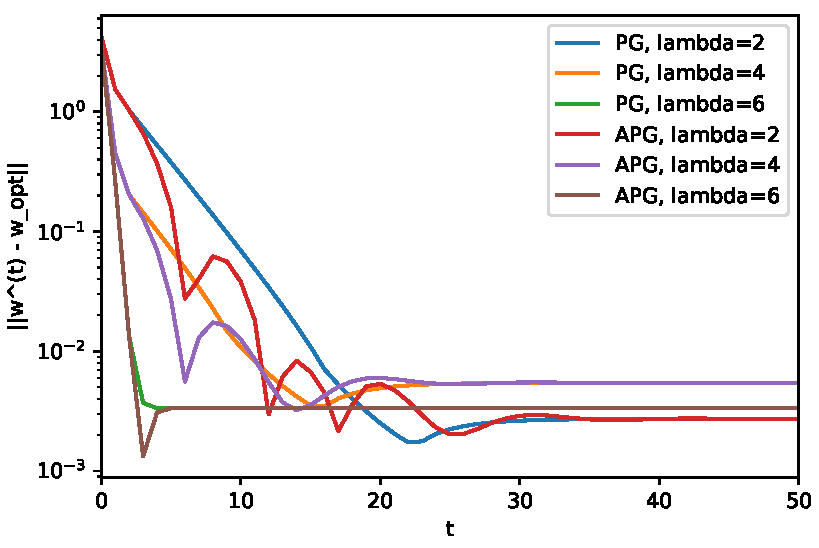
\includegraphics[width=10cm]{figs/p2_lasso_dist.pdf}
 \end{center}
 \caption{\textit{lasso}を用いて学習した時の$||\bm{w}^{(t)} - \hat{\bm{w}}||$の値の変化.
 $\lambda=2,4$の時に一度スコアが上がっているのは,
 $\hat{\bm{w}}$を小数点2桁で打ち切っているためだと考えられる.}
 \label{img:lasso-error}
\end{figure}

\end{document}